\chapter{Implementation}

In this chapter, the previously described components are explained in further details, focusing on how they are implemented, what technologies were used and in addition, some extra fine tunes are presented, which demonstrate the extendability of the open source Grafana.

The source code for the thesis project is available and can be viewed in my GitHub repository.\cite{thesis-repo}

\section{Architecture}

%---
\subsection{Docker}
%---
% https://www.docker.com/resources/what-container

Throughout this project, I run the different components using Docker containers. For this reason, it seems appropriate to briefly introduce this technology.

A container is a standard unit of software that packages up code and all its dependencies so the application runs quickly and reliably from one computing environment to another. A Docker container image is a lightweight, standalone, executable package of software that includes everything needed to run an application: code, runtime, system tools, system libraries and settings.

Container images become containers at runtime and in the case of Docker containers - images become containers when they run on Docker Engine. Available for both Linux and Windows-based applications, containerized software will always run the same, regardless of the infrastructure. Containers isolate software from its environment and ensure that it works uniformly despite differences for instance between development and staging.\cite{docker}


\subsection{Docker Compose}

In order to be able to set up an architecture as the one described in section \ref{arch-design}, I used Docker Compose.

% https://docs.docker.com/compose/

Docker Compose is a tool for defining and running multi-container Docker applications. With Compose, we can use a YAML file to configure application’s services. Then, with a single command, we can create and start all the services from the configuration.\cite{docker-compose}

The \texttt{docker-compose.yml} file for the project can be found in the GitHub repository of the thesis project. It defines all the necessary components with the appropriate configuration.

\vspace{0.5cm}
\begin{minipage}{\linewidth}
	\begin{lstlisting}[language=docker-compose-proxy, caption={Extract of the \texttt{docker-compose.yml}}, label={lst:proxy-docker-compose}]]	
	  proxy:
	    build: ./proxy
	    ports:
	    - 5000:5000
	    restart: always
	    volumes: 
	    - "./proxy/proxy.py:/code/proxy.py"
	\end{lstlisting}
\end{minipage}

\section{Proxy (Gateway)} \label{proxy-impl}

It was established in the design section \ref{proxy-design}, that the main responsibility of the Gateway component is to translate between the JSON data formats used by the RapidMiner Server and the Grafana SimpleJSON data source plugin.

For this task, I had two possibilities. One is to use a tool, which defines the transformation in a declarative way. For example, I could use XLST, which is able to convert a JSON format into another \cite{xslt}. The other option was to implement an own algorithm which handles the transformation of the data format. I chose the latter alternative as the structure of the data was not exceptionally complex, thus it was quite simple to implement a function for this job . The other reason was that this way, I did not have to integrate another tool and call it every time to transform a simple JSON object, which in general reduced the number of possible sources for errors.

% https://www.xml.com/articles/2017/02/14/why-you-should-be-using-xslt-30/

As it was described in section \ref{proxy-design}, the Gateway component must be able to handle requests from Grafana, as well as be able to forward these requests to the RapidMiner Server after the format translation. 

% https://www.palletsprojects.com/p/flask/
% https://realpython.com/python-requests/
For this task, I implemented the Gateway in Python using the \texttt{flask}\cite{flask} and the \texttt{requests}\cite{requests} packages and ran it in a Docker container. Flask is a lightweight web application framework library that enables quick and simple development. Requests can be thought of as the de facto standard for making HTTP requests in Python. It abstracts the complexities of making requests behind a simple API.

%---
\subsection{Endpoints}
%---

As it was explained in section \ref{proxy-design}, the Gateway component has to expose the endpoints that are required by the SimpleJSON data source plugin.

With the \texttt{requests} package, it is quite convenient to implement these endpoints, since we only have to declare a decorated function for each endpoint, as it is shown in the code snippet \ref{lst:proxy-test-conn}.

\vspace{0.5cm}
\begin{minipage}{\linewidth}
\begin{lstlisting}[language=Python, caption={Test the connection to the server}, label={lst:proxy-test-conn}]]
	@app.route('/')
	def check_connection():
	  response = requests.get(server_host)
	    if response.status_code == 200:
	      return 'Server connection OK'
	  return "Server connection error"
\end{lstlisting}
\end{minipage}
%---
\subsubsection{Searching the targets}
%---

To be able to get the names of the available RapidMiner web services, the Gateway component should use the \texttt{/api/rest/service/list} endpoint of the RapidMiner Server. This endpoint returns the names and parameters of the web services in JSON format. The Gateway extracts the names of the services transforms this data into a format that SimpleJSON can understand.

The endpoint is implemented as displayed in the following \ref{lst:proxy-search} code snippet. 

\begin{minipage}{\linewidth}
\begin{lstlisting}[language=Python, caption={Get the names of the web services}, label={lst:proxy-search}]]
@app.route('/search', methods=['POST'])
def search():
  response = requests.get(server_host + '/api/rest/service/list',
                          auth=('admin', 'changeit'))
  webservices_json_list = json.loads(response.text)
  webservice_names = []
  for webservice in webservices_json_list:
    webservice_names.append(webservice['name'])
  return json.dumps(webservice_names)
\end{lstlisting}
\end{minipage}
%---
\subsubsection{Acquiring the parameters}
%---

To get the available parameters of the exposed web services, the Gateway component uses the same endpoint of the RapidMiner Server (\texttt{/api/rest/service/list}), as for searching the targets.

The reason for that these two features are separated, even though they use the same endpoint, is that concerning the Gateway, the functionality of exposing the available targets is required by the SimpleJSON by default while querying the parameters is an extra feature. This means that SimpleJSON expects a specific data format, which only includes the names of the targets. Thus returning the parameters additionally with the targets would break the compatibility between the Gateway component and the SimpleJSON data source plugin.

Acquiring the parameters is implemented the following way, as in the code snippet \ref{lst:proxy-params}.

\begin{minipage}{\linewidth}
	\begin{lstlisting}[language=Python, caption={Get the parameters for a given web service}, label={lst:proxy-params}]]
	@app.route('/parameters', methods=['GET'])
	def parameters():
	  if request.args:
	    args = request.args
	    webserviceName = args.get('webserviceName')
	    if webserviceName == None:
	      raise ValueError('No value provided for "webserviceName"')
	    # get the list of webservices and get the parameters of the one with the name provided in the query
	    response = requests.get(server_host + '/api/rest/service/list',
	    auth=('admin', 'changeit'))
	    webservices_json_list = json.loads(response.text)
	    webservice_params = []
	    for webservice in webservices_json_list:
	      if webservice['name'] == webserviceName:
	        webservice_params = webservice['parameters']
	        break
	    return json.dumps(webservice_params)
	  return 'Please provide a query parameter in the URL'
	\end{lstlisting}
\end{minipage}

%---
\subsubsection{Querying the data}\label{impl-qurying}
%---
When Grafana sends a request to the Gateway component, it specifies the data format, in which it excepts to receive the results. This can be a time series format or a table format which can be seen in the code snippets below.

\begin{minipage}[b]{0.45\linewidth}
	\centering
	\begin{lstlisting}[language=Python, frame=single, numbers=left, mathescape,%
	caption={Time series format}, label=lst:timeseries-format]
	[
	 {
	    "target":"weather_retrieve_process?city=Vancouver",
	    "datapoints":[
	      [284.63, 1573882025382],
	      [284.629, 1573885625382],
	      [284.627, 1573889225382],
	      [284.625, 1573892890284],
	      [284.623, 1573896490284],
	      [284.621, 1575746856319],
	      [284.619, 1575750456319],
	      [284.617, 1575754056319]
	    ]
	 }
	]
	\end{lstlisting}
\end{minipage}
\hspace{0.5cm}
\begin{minipage}[b]{0.45\linewidth}
	\centering
	\begin{lstlisting}[language=Python, frame=single, mathescape,%
	caption={Table format}, label=lst:table-format]
	[
	 {
	   "columns":[
	     {"text":"Month","type":"string"},
	     {"text":"Maxs","type":"number"}
	   ],
	   "rows":[
	     ['2012 October', 1],
	     ['2012 November', 1],
	     ['2012 December', 0],
	     ['2013 January', 0]
	   ],
	   "type":"table"
	 }
	]
	\end{lstlisting}
\end{minipage}

The time series response format contains the target name, which in this case is the name of the RapidMiner web service with an additional parameter attached to it and the data points. The first value in a data point is the actual value, the second is the timestamp in UNIX Epoch time in milliseconds.

The table format describes the name and the type of each column in the \texttt{columns} array. The actual data is in the \texttt{rows} array, every row is defined with a list of values in an order that is correspondent to that of the columns.

%---
\section{Python data source}
%---

As it was mentioned in section \ref{case-study-python-source} and section \ref{proxy-design}, the Python data source communicates with a database and a separate API service in order to prepare the requested data for Grafana.

The Python data source is also connected to Grafana, so it needs to expose the endpoints that are needed by the SimpleJSON data source plugin (discussed in section \ref{simplejson-design}), which are implemented similarly as in the Gateway.

The differing ability of the Python data source compared to the Gateway  component is that it can connect to a MySQL database and an external API to get the requested data by Grafana. To be able to implement these features, I used the \texttt{requests} and the \texttt{mysql.connector} packages along with the \texttt{flask} library, which is needed to be able to send HTTP requests (as in the case of the Gateway component).

% # https://pynative.com/python-mysql-select-query-to-fetch-data/

Reading the data from the MySQL database is implemented as the following pseudo code shows (\ref{lst:mysql-conn}).

\vspace{0.5cm}
\begin{minipage}[b]{\linewidth}
	\centering
	\begin{lstlisting}[language=Python, frame=single, mathescape,%
	caption={Reading data from MySQL}, label=lst:mysql-conn]
	def read_data_from_db():
	  try:
	    connection = mysql.connector.connect(
	      <credentials>
	    )
	    sql_select_records_query = "SELECT * FROM newyork"
	    cursor = connection.cursor()
	    cursor.execute(sql_select_records_query)
	    records = cursor.fetchall()
	    data = []
	    for row in records:
	      record = {
	        <parse data from a record>
	      }
	      data.append(record)
	    return data
	  except Error as error:
	    print("Error reading data from MySQL ", error)
	  finally:
	    <close the connection to the database>
	\end{lstlisting}
\end{minipage}

Getting the recorded information from the 'external' Weather API is much simpler thanks to the level of abstraction the \texttt{requests} package provides. (\ref{lst:weather-conn})

\vspace{0.5cm}
\begin{minipage}[b]{\linewidth}
	\centering
	\begin{lstlisting}[language=Python, frame=single, mathescape,%
	caption={Reading data from the Weather API}, label=lst:weather-conn]
	def get_all_time_records():
	  response = requests.get(weather_api_host + '/all')
	  json_data = json.loads(response.text)
	  return json_data
	\end{lstlisting}
\end{minipage}

After the Python data source possesses the data both from the MySQL database and the Weather API, it aggregates the collected information (\texttt{create\char`_table\char`_data()} function) according to the sample business-logic already discussed in section \ref{case-study-python-source} and then exposes it on its \texttt{/query} endpoint. (\ref{lst:python-query})

\begin{minipage}[b]{\linewidth}
	\centering
	\begin{lstlisting}[language=Python, frame=single, mathescape,%
	caption={Exposing the prepared data}, label=lst:python-query]
	@app.route('/query', methods=['POST'])
	def query():
	  table_data = create_table_data()
	  return json.dumps(table_data)
	\end{lstlisting}
\end{minipage}

%---
\section{Additional features}
%---

After the integration of the two data sources, I implemented some additional features in Grafana to increase its interactivity capabilities. These are mainly developments in the graphical interface, thus they do not affect the already presented architectural model.

%---
\subsection{Customized Grafana Query Editor GUI}
%---

As it was already discussed in section \ref{query-editor}, the Query Editor determines what data Grafana requests from its data sources, hence, what data will be visualized on the panel. 

With the usage of the extra \texttt{/parameters} endpoint of the Gateway component, I implemented the dynamic listing of available parameters for a web service in the Query Editor of the extended SimpleJSON data source plugin.

This means that the user does not have to be familiar with the exact name or amount of the exposed parameters for a web service. When he or she chooses a target to query, Grafana asks the data source to get this information. An example of this dynamic parameter listing can be seen in Figure \ref{fig:dynamic-parameters}. There we have a RapidMiner web service called \texttt{Predicitve\char`_Maintanence\char`_web\char`_service\char`_with\char`_parameters} with two available parameters called \texttt{machineID} and \texttt{sensor1}.

\begin{figure}[h]
	\centering
	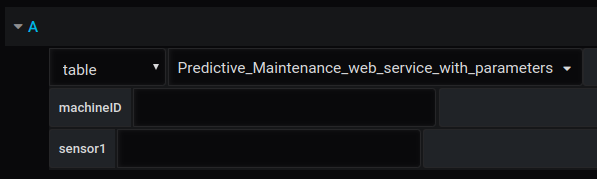
\includegraphics[width=130mm, keepaspectratio]{figures/dynamic-parameters.png}
	\caption{Dynamic listing of available parameters}
	\label{fig:dynamic-parameters}
\end{figure}

%---
\subsection{Dynamic bar chart in Grafana} \label{dynamic-barchart}
%---
% https://github.com/CorpGlory/grafana-graph-panel

In section \ref{grafana-time-range-controls}, it was already discussed, that it is possible to change the time interval of the whole Dashboard by selecting a time range on a Graph Panel.

% https://grafana.com/docs/grafana/latest/features/panels/graph/
The Graph Panel offers other display possibilities as well apart from the graph diagram. It can visualize time series data with bar-charts and histograms \cite{graph-panel}. I focused on the bar-chart format, which groups the data by series and not time, so with this type of diagram, we can display aggregated information about the series. For example the total value, the average, the maximum or the count of the data points.

However, I noticed, that when I change the time range of the Dashboard, these basic statistical indices do not get refreshed based on the new time interval. They keep their original values that were calculated for the whole time series when Grafana received the information from one of its data sources. This phenomenon can be quite misleading in cases when we have multiple Graph Panels with the same querying settings, but with different visualization modes.

To solve this issue, as a part of my thesis project, I successfully extended the built-in Graph Panel, so it calculates the aggregated values only from the data points that are in the time interval of the dashboard. This feature enables a more interactive and valuable insight of the visualized data.

To accomplish this, I used the source code of the built-in Graph Panel configured with the \texttt{webpack} module bundler which enabled the simple integration of this customized panel as a separate plugin for Grafana. \cite{graph-panel-webpack}

%---
\section{Grafana Dashboard} \label{final-dashboard}
%---

As a final, easy to demonstrate result of the integration task of this project, I created a Dashboard in Grafana to display the collected data from various sources that can be seen in Figure \ref{fig:dashboard-final}. As it was already expressed in chapter \ref{case-study}, I used a sample data set containing information about weather in different cities in order to be able to visualize the results of the created architecture.

\begin{figure}[h]
	\centering
	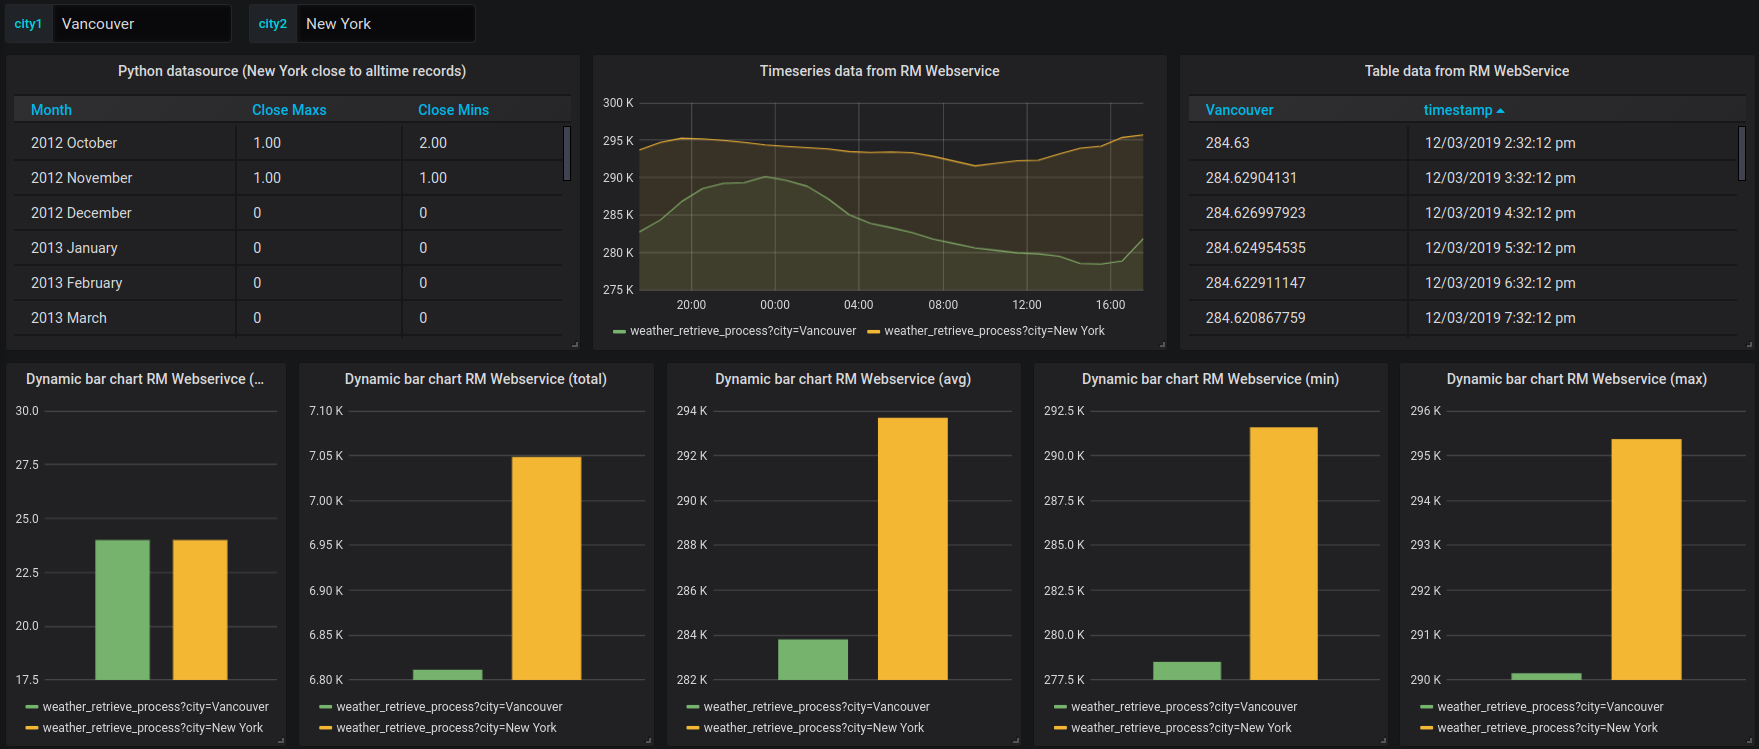
\includegraphics[width=\linewidth, keepaspectratio]{figures/final-dashboard.png}
	\caption{Dashboard showing the results}
	\label{fig:dashboard-final}
\end{figure}

The Graph Panel in the middle shows the same two time series data as the five bar-chart diagrams that display some basic statistical indices in a time-dependent manner as discussed before in section \ref{dynamic-barchart} introducing the dynamic bar-chart.

All the visualized data on this Dashboard comes from the RapidMiner Server component through exposed web services, expect for the table in the top-left corner, which shows recorded information originating from the Python data source unit.

On the top of the Dashboard, two templating variables can be seen, which determine the two cities that we use to filter the displayed data.
